% Options for packages loaded elsewhere
\PassOptionsToPackage{unicode}{hyperref}
\PassOptionsToPackage{hyphens}{url}
%
\documentclass[
]{book}
\usepackage{amsmath,amssymb}
\usepackage{iftex}
\ifPDFTeX
  \usepackage[T1]{fontenc}
  \usepackage[utf8]{inputenc}
  \usepackage{textcomp} % provide euro and other symbols
\else % if luatex or xetex
  \usepackage{unicode-math} % this also loads fontspec
  \defaultfontfeatures{Scale=MatchLowercase}
  \defaultfontfeatures[\rmfamily]{Ligatures=TeX,Scale=1}
\fi
\usepackage{lmodern}
\ifPDFTeX\else
  % xetex/luatex font selection
\fi
% Use upquote if available, for straight quotes in verbatim environments
\IfFileExists{upquote.sty}{\usepackage{upquote}}{}
\IfFileExists{microtype.sty}{% use microtype if available
  \usepackage[]{microtype}
  \UseMicrotypeSet[protrusion]{basicmath} % disable protrusion for tt fonts
}{}
\makeatletter
\@ifundefined{KOMAClassName}{% if non-KOMA class
  \IfFileExists{parskip.sty}{%
    \usepackage{parskip}
  }{% else
    \setlength{\parindent}{0pt}
    \setlength{\parskip}{6pt plus 2pt minus 1pt}}
}{% if KOMA class
  \KOMAoptions{parskip=half}}
\makeatother
\usepackage{xcolor}
\usepackage{color}
\usepackage{fancyvrb}
\newcommand{\VerbBar}{|}
\newcommand{\VERB}{\Verb[commandchars=\\\{\}]}
\DefineVerbatimEnvironment{Highlighting}{Verbatim}{commandchars=\\\{\}}
% Add ',fontsize=\small' for more characters per line
\usepackage{framed}
\definecolor{shadecolor}{RGB}{248,248,248}
\newenvironment{Shaded}{\begin{snugshade}}{\end{snugshade}}
\newcommand{\AlertTok}[1]{\textcolor[rgb]{0.94,0.16,0.16}{#1}}
\newcommand{\AnnotationTok}[1]{\textcolor[rgb]{0.56,0.35,0.01}{\textbf{\textit{#1}}}}
\newcommand{\AttributeTok}[1]{\textcolor[rgb]{0.13,0.29,0.53}{#1}}
\newcommand{\BaseNTok}[1]{\textcolor[rgb]{0.00,0.00,0.81}{#1}}
\newcommand{\BuiltInTok}[1]{#1}
\newcommand{\CharTok}[1]{\textcolor[rgb]{0.31,0.60,0.02}{#1}}
\newcommand{\CommentTok}[1]{\textcolor[rgb]{0.56,0.35,0.01}{\textit{#1}}}
\newcommand{\CommentVarTok}[1]{\textcolor[rgb]{0.56,0.35,0.01}{\textbf{\textit{#1}}}}
\newcommand{\ConstantTok}[1]{\textcolor[rgb]{0.56,0.35,0.01}{#1}}
\newcommand{\ControlFlowTok}[1]{\textcolor[rgb]{0.13,0.29,0.53}{\textbf{#1}}}
\newcommand{\DataTypeTok}[1]{\textcolor[rgb]{0.13,0.29,0.53}{#1}}
\newcommand{\DecValTok}[1]{\textcolor[rgb]{0.00,0.00,0.81}{#1}}
\newcommand{\DocumentationTok}[1]{\textcolor[rgb]{0.56,0.35,0.01}{\textbf{\textit{#1}}}}
\newcommand{\ErrorTok}[1]{\textcolor[rgb]{0.64,0.00,0.00}{\textbf{#1}}}
\newcommand{\ExtensionTok}[1]{#1}
\newcommand{\FloatTok}[1]{\textcolor[rgb]{0.00,0.00,0.81}{#1}}
\newcommand{\FunctionTok}[1]{\textcolor[rgb]{0.13,0.29,0.53}{\textbf{#1}}}
\newcommand{\ImportTok}[1]{#1}
\newcommand{\InformationTok}[1]{\textcolor[rgb]{0.56,0.35,0.01}{\textbf{\textit{#1}}}}
\newcommand{\KeywordTok}[1]{\textcolor[rgb]{0.13,0.29,0.53}{\textbf{#1}}}
\newcommand{\NormalTok}[1]{#1}
\newcommand{\OperatorTok}[1]{\textcolor[rgb]{0.81,0.36,0.00}{\textbf{#1}}}
\newcommand{\OtherTok}[1]{\textcolor[rgb]{0.56,0.35,0.01}{#1}}
\newcommand{\PreprocessorTok}[1]{\textcolor[rgb]{0.56,0.35,0.01}{\textit{#1}}}
\newcommand{\RegionMarkerTok}[1]{#1}
\newcommand{\SpecialCharTok}[1]{\textcolor[rgb]{0.81,0.36,0.00}{\textbf{#1}}}
\newcommand{\SpecialStringTok}[1]{\textcolor[rgb]{0.31,0.60,0.02}{#1}}
\newcommand{\StringTok}[1]{\textcolor[rgb]{0.31,0.60,0.02}{#1}}
\newcommand{\VariableTok}[1]{\textcolor[rgb]{0.00,0.00,0.00}{#1}}
\newcommand{\VerbatimStringTok}[1]{\textcolor[rgb]{0.31,0.60,0.02}{#1}}
\newcommand{\WarningTok}[1]{\textcolor[rgb]{0.56,0.35,0.01}{\textbf{\textit{#1}}}}
\usepackage{longtable,booktabs,array}
\usepackage{calc} % for calculating minipage widths
% Correct order of tables after \paragraph or \subparagraph
\usepackage{etoolbox}
\makeatletter
\patchcmd\longtable{\par}{\if@noskipsec\mbox{}\fi\par}{}{}
\makeatother
% Allow footnotes in longtable head/foot
\IfFileExists{footnotehyper.sty}{\usepackage{footnotehyper}}{\usepackage{footnote}}
\makesavenoteenv{longtable}
\usepackage{graphicx}
\makeatletter
\def\maxwidth{\ifdim\Gin@nat@width>\linewidth\linewidth\else\Gin@nat@width\fi}
\def\maxheight{\ifdim\Gin@nat@height>\textheight\textheight\else\Gin@nat@height\fi}
\makeatother
% Scale images if necessary, so that they will not overflow the page
% margins by default, and it is still possible to overwrite the defaults
% using explicit options in \includegraphics[width, height, ...]{}
\setkeys{Gin}{width=\maxwidth,height=\maxheight,keepaspectratio}
% Set default figure placement to htbp
\makeatletter
\def\fps@figure{htbp}
\makeatother
\setlength{\emergencystretch}{3em} % prevent overfull lines
\providecommand{\tightlist}{%
  \setlength{\itemsep}{0pt}\setlength{\parskip}{0pt}}
\setcounter{secnumdepth}{5}
\usepackage{booktabs}
\usepackage{amsthm}
\usepackage{natbib} % Required for bibliography
\usepackage{csquotes} % Provides advanced quoting and citation features

% Define the citation-note environment if it's required
\newenvironment{citation-note}
    {\begin{quote}\itshape}
    {\end{quote}}

\makeatletter
\def\thm@space@setup{%
  \thm@preskip=8pt plus 2pt minus 4pt
  \thm@postskip=\thm@preskip
}
\makeatother
\ifLuaTeX
  \usepackage{selnolig}  % disable illegal ligatures
\fi
\usepackage[]{natbib}
\bibliographystyle{plainnat}
\usepackage{bookmark}
\IfFileExists{xurl.sty}{\usepackage{xurl}}{} % add URL line breaks if available
\urlstyle{same}
\hypersetup{
  pdftitle={RMC Filter Evaluation (Continuation) Toolbox Technical Manual},
  pdfauthor={Adam C. Gohs},
  hidelinks,
  pdfcreator={LaTeX via pandoc}}

\title{RMC Filter Evaluation (Continuation) Toolbox Technical Manual}
\author{Adam C. Gohs}
\date{Last updated: 2025-01-23}

\begin{document}
\maketitle

{
\setcounter{tocdepth}{1}
\tableofcontents
}
\chapter*{Preface}\label{preface}
\addcontentsline{toc}{chapter}{Preface}

The Risk Management Center (RMC) of the U.S. Army Corps of Engineers (USACE) has developed a suite of Microsoft Excel spreadsheets to support risk assessments for dam and levee safety. Each analysis suite is composed of multiple toolboxes (Microsoft Excel workbooks), and each toolbox contains multiple spreadsheet tools or calculation worksheets (Microsoft Excel worksheets). The RMC Filter Evaluation (Continuation) Toolbox is part of the RMC Internal Erosion Suite.

The spreadsheet tools contained in this toolbox assess the particle retention and permeability criteria for filter materials It includes modern no erosion filter design criteria, Foster and Fell (2001) method for filters that do not meet modern filter design criteria, and the Fell and Foster (2023) method for ``continuing erosion'' condition for constricted exits.

\subsection*{How to Cite This Guide}\label{how-to-cite-this-guide}
\addcontentsline{toc}{subsection}{How to Cite This Guide}

If you would like to cite this User's Guide, please use the following format:

\begin{citation-note}
A. C. Gohs, \emph{RMC Filter Evaluation (Continuation) Toolbox Technical
Manual}, Lakewood, CO: U.S. Army Corps of Engineers, Risk Management
Center, 2024. Accessed on {\textless enter current date
here\textgreater{}}.
\end{citation-note}

\chapter{Introduction}\label{introduction}

The Risk Management Center (RMC) of the U.S. Army Corps of Engineers (USACE) has developed a suite of Microsoft Excel spreadsheets to support risk assessments for dam and levee safety. Each analysis suite is composed of multiple toolboxes (Microsoft Excel workbooks), and each toolbox contains multiple spreadsheet tools or calculation worksheets (Microsoft Excel worksheets). The RMC Filter Evaluation (Continuation) Toolbox is part of the RMC Internal Erosion Suite.

The information from these spreadsheet tools, along with other pertinent information, informs judgment when developing a list of more and less likely factors and estimating probabilities. USACE best practice for estimating probabilities is to use the best available and multiple methods, but all final probabilities are estimated using team elicitation based on the totality and strength of the evidence.

The RMC continuously works to improve the performance of RMC software; report possible bugs directly to the RMC at the address listed below. Ideally, report suspected errors in written form with a description of the problem and the steps that lead to its occurrence. Suggestions for improvement are also welcomed.

U.S. Army Corps of Engineers
Institute for Water Resources
Risk Management Center
\href{mailto:RMC.software@usace.army.mil}{\nolinkurl{RMC.software@usace.army.mil}}

\chapter{Terms and Conditions for Use}\label{terms-and-conditions-for-use}

By using Institute for Water Resources (IWR) software, users voluntarily accept the following terms and conditions. Users that do not agree to these terms and conditions should uninstall the IWR software and return any program materials to IWR and its technical centers. If users downloaded the software and do not have disk media, delete all copies and cease using the software.

\section{Terms and Conditions for Use of Institute for Water Resources Software}\label{terms-and-conditions-for-use-of-institute-for-water-resources-software}

The United States Government, U.S. Army Corps of Engineers, Institute for Water Resources (``IWR''), and IWR's technical centers including the Risk Management Center (``RMC'') and Hydrologic Engineering Center (``HEC'') grant to the user the rights to install ``IWR Software'' (either from a disk copy obtained from IWR and IWR's technical centers, a distributor or another user or by downloading it from a network) and to use, copy and/or distribute copies of the IWR Software to other users, subject to the following Terms and Conditions of Use:

\begin{itemize}
\item
  All copies of the IWR Software received or reproduced by or for user pursuant to the authority of this Terms and Conditions of Use will be and remain the property of IWR.
\item
  User may reproduce and distribute the IWR Software provided that the recipient agrees to the Terms and Conditions for Use noted herein.
\item
  IWR and IWR's technical centers are solely responsible for the content of the IWR Software. The IWR Software may not be modified, abridged, decompiled, disassembled, unobfuscated or reverse engineered. The user is solely responsible for the content, interactions, and effects of any and all amendments, if present, whether they be extension modules, language resource bundles, scripts, or any other amendment.
\item
  The name of the IWR Software must not be used to endorse or promote products derived from the IWR Software. Products derived from the IWR Software may not be called the IWR Software nor may any part of the IWR Software name appear within the name of derived products.
\item
  No part of this Terms and Conditions for Use may be modified, deleted or obliterated from the IWR Software.
\item
  No part of the IWR Software may be exported or re-exported in contravention of U.S. export laws or regulations.
\end{itemize}

\section{Waiver of Warranty}\label{waiver-of-warranty}

THE UNITED STATES GOVERNMENT AND ITS AGENCIES, OFFICIALS, REPRESENTATIVES, AND EMPLOYEES, INCLUDING ITS CONTRACTORS AND SUPPLIERS PROVIDE THE IWR SOFTWARE ``AS IS,'' WITHOUT ANY WARRANTY OR CONDITION, EXPRESS, IMPLIED OR STATUTORY, AND SPECIFICALLY DISCLAIM ANY IMPLIED WARRANTIES OF TITLE, MERCHANTABILITY, FITNESS FOR A PARTICULAR PURPOSE AND NON-INFRINGEMENT. Depending on state law, the foregoing disclaimer may not apply to you, and you may also have other legal rights that vary from state to state.

\section{Limitation of Liability}\label{limitation-of-liability}

IN NO EVENT SHALL THE UNITED STATES GOVERNMENT AND ITS AGENCIES, OFFICIALS, REPRESENTATIVES, AND EMPLOYEES, INCLUDING ITS CONTRACTORS AND SUPPLIERS, BE LIABLE FOR LOST PROFITS OR ANY SPECIAL, INCIDENTAL OR CONSEQUENTIAL DAMAGES ARISING OUT OF OR IN CONNECTION WITH USE OF THE IWR SOFTWARE REGARDLESS OF CAUSE, INCLUDING NEGLIGENCE. THE UNITED STATES GOVERNMENT'S LIABILITY, AND THE LIABILITY OF ITS AGENCIES, OFFICIALS, REPRESENTATIVES, AND EMPLOYEES, INCLUDING ITS CONTRACTORS AND SUPPLIERS, TO YOU OR ANY THIRD PARTIES IN ANY CIRCUMSTANCE IS LIMITED TO THE REPLACEMENT OF CERTIFIED COPIES OF THE IWR SOFTWARE WITH IDENTIFIED ERRORS CORRECTED. Depending on state law, the above limitation or exclusion may not apply to you.

\section{Indemnity}\label{indemnity}

As a voluntary user of the IWR Software you agree to indemnify and hold the United States Government, and its agencies, officials, representatives, and employees, including its contractors and suppliers, harmless from any claim or demand, including reasonable attorneys' fees, made by any third party due to or arising out of your use of the IWR Software or breach of this Agreement or your violation of any law or the rights of a third party.

\chapter{General Overview}\label{general-overview}

\section{Getting Started}\label{getting-started}

Copy or download the toolbox file to the computer. To open the toolbox file, either:

\begin{itemize}
\item
  Find the file on the computer and double-click it. This opens the file in Microsoft Excel.
\item
  Open Microsoft Excel and use the application to open the file: Once Microsoft Excel is open, go to the File menu at the top of the window and select Open.
\end{itemize}

The toolbox is an Excel binary workbook (.xlsb) that uses macros. You may need to enable the macros, either before opening the file or by clicking ``Enable Content'' in the yellow Security Warning message bar with a shield icon that appears after the file is opened. The actual message in the message bar will vary depending on the computer's settings and installed add-ins. Figure \ref{fig:figure-1} displays examples of different wordings that may appear in the message bar.

\begin{Shaded}
\begin{Highlighting}[]
\NormalTok{knitr}\SpecialCharTok{::}\FunctionTok{include\_graphics}\NormalTok{(}\StringTok{"images/figure1.png"}\NormalTok{)}
\end{Highlighting}
\end{Shaded}

\begin{figure}

{\centering 
\includegraphics{images/figure1} 

}

\caption{Security warning message bars with the "Enable Content" option to enable macros.}\label{fig:figure-1}
\end{figure}

\section{Organization}\label{organization}

Although the toolbox does not provide a calculation cover sheet, adding one is strongly recommended. A calculation cover sheet captures project information, a description and purpose of the calculation, the assumptions for critical input parameters, a summary of the major conclusion and results, and a revision history.

Each toolbox has a similar appearance and organizational structure:

\begin{itemize}
\item
  The first worksheet, About, summarizes the purpose of the toolbox and gives contact information for the RMC software development team.
\item
  The second worksheet, Terms and Conditions, contains the terms and conditions for use of the toolbox (IWR software).
\item
  The third worksheet, Version History, contains the revision history. Semantic versioning is used in the format of MAJOR.MINOR.PATCH:

  \begin{itemize}
  \item
    MAJOR - significant worksheet changes not compatible with previous versions.
  \item
    MINOR - additional features or enhancements that do not fundamentally change the calculations.
  \item
    PATCH - backward-compatible bug fixes.
  \end{itemize}
\item
  The fourth worksheet, References, lists the references cited for each calculation worksheet.
\end{itemize}

The workbook and worksheets are not protected to prevent unwanted changes. However, because the toolbox has user-defined functions (UDFs) and subroutines in Visual Basic, you cannot directly copy worksheets to another workbook without potentially losing functionality. A note in a bold red font at the upper right margin indicates if the selected worksheet includes such features.

At the top of each calculation worksheet, input information for the preparer and checker for quality control (QC) documentation and the calculation title in case multiple copies of the worksheet are created for different analysis scenarios (Figure \ref{fig:figure-2}). The footer of each calculation worksheet contains the version number, which can be cross-referenced with the revision history on the third worksheet.

\begin{Shaded}
\begin{Highlighting}[]
\NormalTok{knitr}\SpecialCharTok{::}\FunctionTok{include\_graphics}\NormalTok{(}\StringTok{"images/figure2.png"}\NormalTok{)}
\end{Highlighting}
\end{Shaded}

\begin{figure}

{\centering 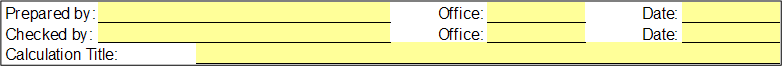
\includegraphics{images/figure2} 

}

\caption{Calculation worksheet heading.}\label{fig:figure-2}
\end{figure}

User-specified input includes values and selections from drop-down lists. User input cells are light yellow, and these cells are unprotected. When cells use drop-down lists, a note in blue font in the right margin of the row alerts the user to use the drop-down list. Conditional formatting applies a gray background to cells that are not based on a user selection. When a user-specified value or calculated value is outside of acceptable ranges, the cell is orange to indicate caution to the user.

All units for user-specified input values are clearly labeled. Most user-specified input values use English units. However, values may be in metric where metric units are more common in practice (e.g., particle size in millimeters or permeability in centimeters per second). The toolbox may convert English units to metric units to perform some calculations or if required for a specific formula based on the reference material for the equation.

If the calculation worksheet is a function of headwater level, up to seven headwater and tailwater levels may be specified at the top of the worksheet. Tailwater may be required to calculate the net hydraulic head and hydraulic gradient. Specify the elevation datum by selecting one of three options from the drop-down list: ft-NAVD88, ft-NGVD29, and Other. The two datum selections include English units of length (feet). If Other is selected, provide a user-specified datum along with feet (e.g., ft-MSL {[}Mean Sea Level{]}). Figure \ref{fig:figure-3}, Figure \ref{fig:figure-4}, and Figure \ref{fig:figure-5} illustrate the three possible scenarios.

\begin{Shaded}
\begin{Highlighting}[]
\NormalTok{knitr}\SpecialCharTok{::}\FunctionTok{include\_graphics}\NormalTok{(}\StringTok{"images/figure3.png"}\NormalTok{)}
\end{Highlighting}
\end{Shaded}

\begin{figure}

{\centering 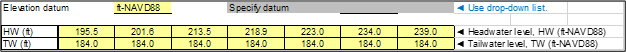
\includegraphics{images/figure3} 

}

\caption{Headwater and tailwater input: NAVD88.}\label{fig:figure-3}
\end{figure}

\begin{Shaded}
\begin{Highlighting}[]
\NormalTok{knitr}\SpecialCharTok{::}\FunctionTok{include\_graphics}\NormalTok{(}\StringTok{"images/figure4.png"}\NormalTok{)}
\end{Highlighting}
\end{Shaded}

\begin{figure}

{\centering 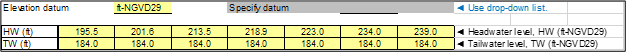
\includegraphics{images/figure4} 

}

\caption{Headwater and tailwater input: NGVD29.}\label{fig:figure-4}
\end{figure}

\begin{Shaded}
\begin{Highlighting}[]
\NormalTok{knitr}\SpecialCharTok{::}\FunctionTok{include\_graphics}\NormalTok{(}\StringTok{"images/figure5.png"}\NormalTok{)}
\end{Highlighting}
\end{Shaded}

\begin{figure}

{\centering 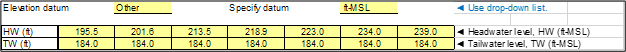
\includegraphics{images/figure5} 

}

\caption{Headwater and tailwater input: User-specified datum.}\label{fig:figure-5}
\end{figure}

Most calculation worksheets break down complex analysis into computational steps following a logical sequence (Figure \ref{fig:figure-6}). Some simpler worksheets do not have steps. Generally, different methodologies are unique worksheets. Some worksheets may include multiple methodologies, which are labeled as options (Figure \ref{fig:figure-7}).

\begin{Shaded}
\begin{Highlighting}[]
\NormalTok{knitr}\SpecialCharTok{::}\FunctionTok{include\_graphics}\NormalTok{(}\StringTok{"images/figure6.png"}\NormalTok{)}
\end{Highlighting}
\end{Shaded}

\begin{figure}

{\centering 
\includegraphics{images/figure6} 

}

\caption{Example of step banner.}\label{fig:figure-6}
\end{figure}

\begin{Shaded}
\begin{Highlighting}[]
\NormalTok{knitr}\SpecialCharTok{::}\FunctionTok{include\_graphics}\NormalTok{(}\StringTok{"images/figure7.png"}\NormalTok{)}
\end{Highlighting}
\end{Shaded}

\begin{figure}

{\centering 
\includegraphics{images/figure7} 

}

\caption{Example of option banner.}\label{fig:figure-7}
\end{figure}

Some calculation worksheets can perform either a deterministic or probabilistic analysis. Although not required to perform a probabilistic analysis, Palisade \citet{RISK} software (standalone version or as part of the Palisade DecisionTools Suite) can customize the probabilistic analysis. A note appears in a bold red font at the upper right-hand margin of a calculation worksheet indicating if this feature is included with the toolbox.

User notes generally appear in the right margin of each calculation worksheet. Some notes are in blue or red font for heightened awareness. These notes include references to source materials for equations, figures, tables, pages, etc. If the RMC modified the source material, the reference citation says ``adapted from'' instead of ``from.''

Tabular and/or graphical summaries are generally the primary output of the toolbox. The UDFs in the PlotScale module change the minimum and maximum values of the x-axis and y-axis for charts. If the calculation worksheet is a function of headwater level, you can define up to five headwater levels of interest and plot them as vertical reference lines. By selecting the chart and then selecting the Filter icon to display the filter pane, you can choose which data series to display. This is useful when computing the results from multiple methodologies, but not all are applicable or desired to display.

\chapter{Background}\label{background}

Once erosion initiates, it continues unless the eroding forces are reduced or migrating eroded particles are impeded. Continuation is the phase of internal erosion where the relationship of the particle-size distribution between the base soil (core) and the filters or adjacent materials controls whether erosion will continue.

Filters are designed to prevent particle movement from intergranular seepage flow where defects are present in a base soil or seepage water flows through pore spaces of a soil mass in an embankment or foundation. A properly designed filter prevents movement of base soils by seepage forces at a discharge face. The filter supports the discharge face such that bridging between closely spaced contact points prevents any movement of base soil particles into the filter. The filter is also sufficiently coarse to allow seepage water to escape freely. Figure \ref{fig:figure-8} illustrates how the filter, in contact with the soil discharge face, supports and prevents soil movement.

\begin{Shaded}
\begin{Highlighting}[]
\NormalTok{knitr}\SpecialCharTok{::}\FunctionTok{include\_graphics}\NormalTok{(}\StringTok{"images/figure8.png"}\NormalTok{)}
\end{Highlighting}
\end{Shaded}

\begin{figure}

{\centering 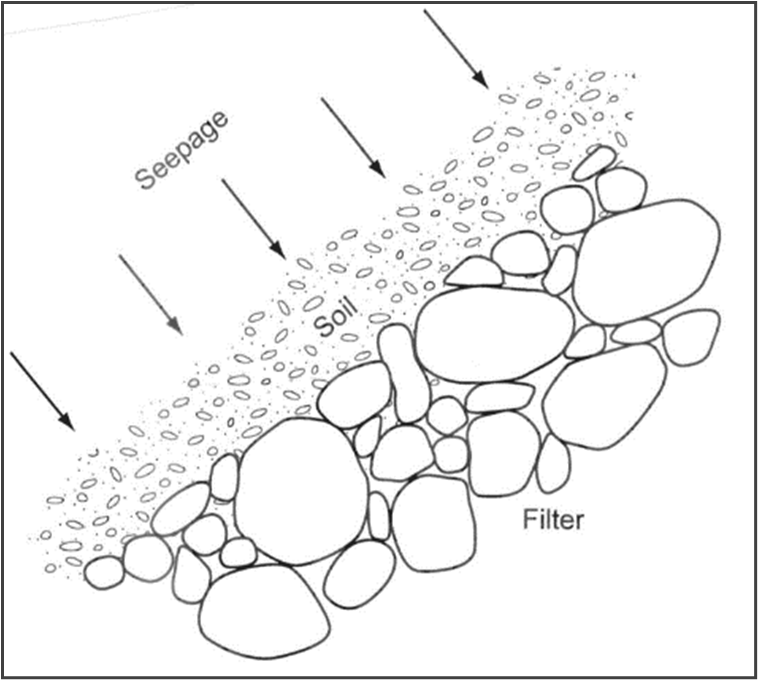
\includegraphics{images/figure8} 

}

\caption{Schematic of filter providing particle retention (FEMA 2011).}\label{fig:figure-8}
\end{figure}

The Federal Emergency Management Agency (FEMA) (2011) defines a filter as a soil gradation that meets both particle retention and drainage criteria. The term drain refers to a soil gradation that is typically a second stage to the first-stage filter and conveys larger amounts of seepage. This toolbox assesses the particle retention and permeability criteria of filters to inform the likelihood of continuation of erosion. The procedures for evaluating particle retention can be for single-stage and multi-stage filters. For multi-stage filters, repeat the procedure for each zone boundary progressing from the finest to the coarsest-grained filter material.

In their published literature, Terzaghi and Sherard used a lowercase ``d'' to represent the particle size (diameter) of the base soil and an uppercase ``D'' for the particle size (diameter) of the filter material. This nomenclature is still commonly used but can be confusing when designing or evaluating two-stage filters since the filter from the first stage becomes the base for the second stage. Therefore, the toolbox uses the following nomenclature:

-\emph{D\textsubscript{XX}Y}, where \emph{D} = particle size (diameter)

\begin{itemize}
\item
  \emph{XX} = percentage passing by weight of particles finer than \emph{D}
\item
  \emph{Y} = material designation (either \emph{B} = base, \emph{F} = first-stage filter, \emph{E} = second-stage envelope, or other drainage element).
\end{itemize}

  \bibliography{book.bib}

\end{document}
